\documentclass[12pt,a4paper]{report}

\usepackage[utf8]{inputenc}
\usepackage[T1]{fontenc}
\usepackage[left=2cm,right=2cm,top=2cm,bottom=2cm]{geometry}
\usepackage{pgfplots}
\usepackage{graphicx}
\usepackage{tikz}
\usepackage{amsmath}
\usepackage{tabularx}
\usepackage{charter}
\usepackage{ngerman}
\usepackage{subfiles}
\usetikzlibrary{decorations.pathmorphing}

\pgfplotsset{compat=1.18}

\title{Physik Oberstufe}
\author{Ben Siebert}
\date{Grundkurs 2023-2025 NRW}

\setcounter{tocdepth}{6}

\begin{document}
	\maketitle
	\tableofcontents

	\chapter{Elektrizitätslehre}
	
	\section{Spezielle Betrachtung zur Elektronenablenkröhre}
	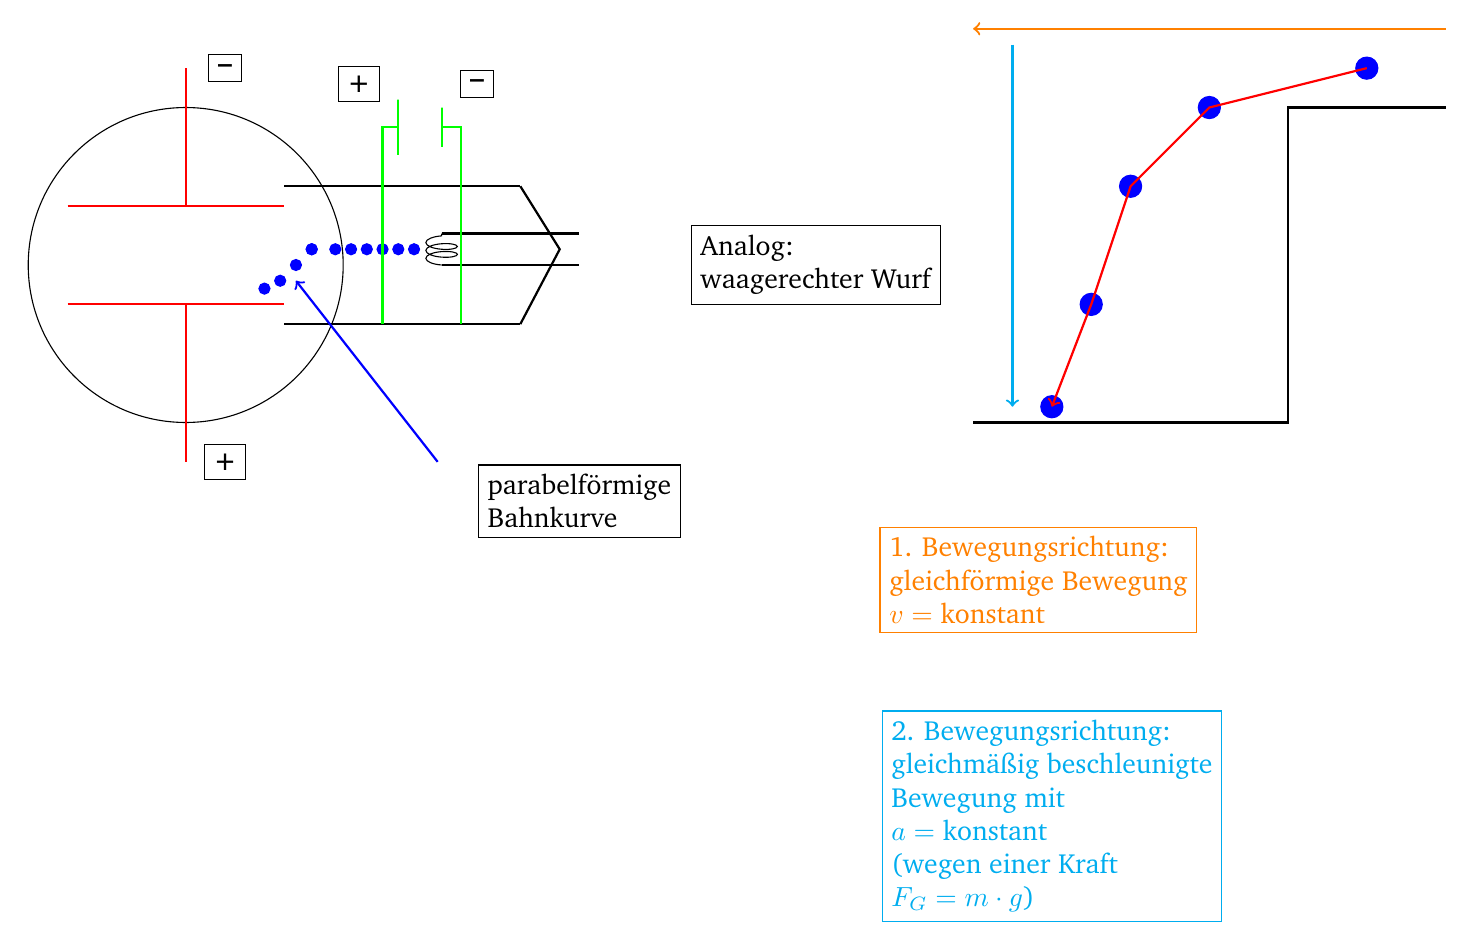
\begin{tikzpicture}
		\draw (1,0) circle (2cm);
		\draw[red,thick] (-0.5,-0.5) -- (2.25,-0.5);
		\draw[red,thick] (-0.5,0.75) -- (2.25,0.75);
		\draw[red,thick] (1,-0.5)  -- (1,-2.5);
		\draw[red,thick] (1,0.75)  -- (1,2.5);
		\node[draw,align=left] at (1.5,2.5) {\textbf{--}};				
		\node[draw,align=left] at (1.5,-2.5) {\textbf{+}};
		\draw[black,thick] (2.25,1) -- (5.25,1);
		\draw[black,thick] (2.25,-0.75) -- (5.25,-0.75);		
		\draw[black,thick] (5.25,1) -- (5.75,0.2) -- (5.25,-0.75);
		\draw[black,thick] (4.25,0.4) -- (6,0.4);
		\draw[black,thick] (4.25,0) -- (6,0);
		\draw[decoration={aspect=0.3,segment length=1mm,amplitude=2mm,coil},decorate] (4.25,0) -- (4.25,0.4);
		\filldraw[blue] (3.9,0.2) circle (2pt);
		\filldraw[blue] (3.7,0.2) circle (2pt);
		\filldraw[blue] (3.5,0.2) circle (2pt);
		\filldraw[blue] (3.3,0.2) circle (2pt);
		\filldraw[blue] (3.1,0.2) circle (2pt);
		\filldraw[blue] (2.9,0.2) circle (2pt);
		\filldraw[blue] (2.6,0.2) circle (2pt);		
		\filldraw[blue] (2.6,0.2) circle (2pt);		
		\filldraw[blue] (2.4,0) circle (2pt);
		\filldraw[blue] (2.2,-0.2) circle (2pt);
		\filldraw[blue] (2,-0.3) circle (2pt);
		\draw[thick,blue,<-] (2.4,-0.2) -- (4.2,-2.5);
		\node[draw,align=left] at (6,-3) {parabelförmige\\ Bahnkurve};
		
		\draw[green,thick] (3.5,-0.75) -- (3.5,1.75) -- (3.7,1.75) -- (3.7,2.1) -- (3.7,1.4);
		\draw[green,thick] (4.5,-0.75) -- (4.5,1.75) -- (4.25,1.75) -- (4.25,2) -- (4.25,1.5);
		\node[draw,align=left] at (3.2,2.3) {\textbf{+}};
    	\node[draw,align=left] at (4.7,2.3) {\textbf{--}};
    	\node[draw,align=left] at (9,0) {Analog: \\ waagerechter Wurf};
    	\draw[black,thick] (11,-2) -- (15,-2) -- (15,2) -- (17,2);
    	\filldraw[blue] (16,2.5) circle (4pt);
    	\filldraw[blue] (14,2) circle (4pt);
    	\filldraw[blue] (13,1) circle (4pt);
    	\filldraw[blue] (12.5,-0.5) circle (4pt);
    	\filldraw[blue] (12,-1.8) circle (4pt);
    	\draw[thick,red,smooth,->] (16,2.5) -- (14,2) -- (13,1) -- (12.5,-0.5) -- (12,-1.8);
    	\draw[thick,orange,->] (17,3) -- (11,3);
    	\draw[thick,cyan,->] (11.5,2.8) -- (11.5,-1.8);
    	\node[draw,align=left,orange] at (11.83,-4) {1. Bewegungsrichtung:\\ gleichförmige Bewegung\\ $v=\text{konstant}$};
    	\node[draw,align=left,cyan] at (12,-7) {2. Bewegungsrichtung:\\ gleichmäßig beschleunigte\\ Bewegung mit \\ $a=\text{konstant}$\\ (wegen einer Kraft \\ $F_G=m\cdot g$)};
	\end{tikzpicture}
	\\\\
	Daraus folgt, dass es eine Kraft $F_E$ (elektrische Kraft) geben muss, damit eine parabelförmige Bahn entsteht $\to$ es gibt eine kraft $F_E$ im \dq elektrischen Raum\dq\ :
	\begin{align*}
	    g &\to E (\text{elektrische Feldstärke}) \\
	    m &\to Q (\text{Ladung}) \\
	    F_E &= E \cdot Q
	\end{align*}
	$E$ beschreibt dabei die Stärke des Feldes zwischen den geladenen Platten und $Q$ die Ladung des Elektrons.
	
	\subsection{Teil 1: Betrachtung der Stärke des Feldes}
	
	\paragraph{a)}\mbox{} \\
	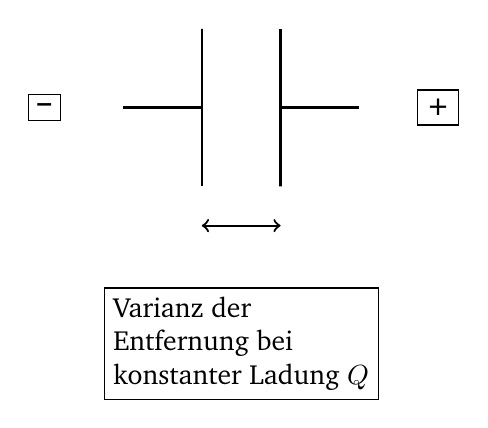
\begin{tikzpicture}
	    \draw[black,thick] (2,0) -- (3,0) -- (3,1) -- (3,-1);
	    \node[draw,align=left] at (1,0) {\textbf{--}};
	    \draw[black,thick] (4,1) -- (4,-1) -- (4,0) -- (5,0);
	    \node[draw,align=left] at (6,0) {\textbf{+}};
	    \draw[black,thick,<->] (3,-1.5) -- (4,-1.5);
	    \node[draw,align=left] at (3.5,-3) {Varianz der \\ Entfernung bei \\ konstanter Ladung $Q$};
	\end{tikzpicture}
	\\\\
	\begin{tabularx}{\textwidth}{|X|X|X|X|X|X|}
        \hline
        \textbf{d/cm} & 1 & 3 & 5 & 7 & 10 \\
        \hline
        \textbf{E/$\frac{kV}{m}$} & 300 & 210 & 160 & 100 & 80 \\
        \hline
	\end{tabularx}
	\\[1cm]
	\begin{tikzpicture}
	    \begin{axis}[
	        axis lines = left,
	        ylabel = $E/\frac{kV}{m}$,
	        xlabel = $d/cm$
	    ]
	        \addplot[
	            color=blue,
	            mark=square,
	            smooth,
	            thick
	        ] coordinates {
	            (1,300)(3,210)(5,160)(7,100)(10,80)
	        };
	    \end{axis}
	\end{tikzpicture}
	\\[1cm]
	Daraus folgt, dass $E$ antiproportional zu $d$ ist:
	\begin{align*}
	    E &\sim \frac{1}{d}
	\end{align*}
	\paragraph{b)}\mbox{} \\
	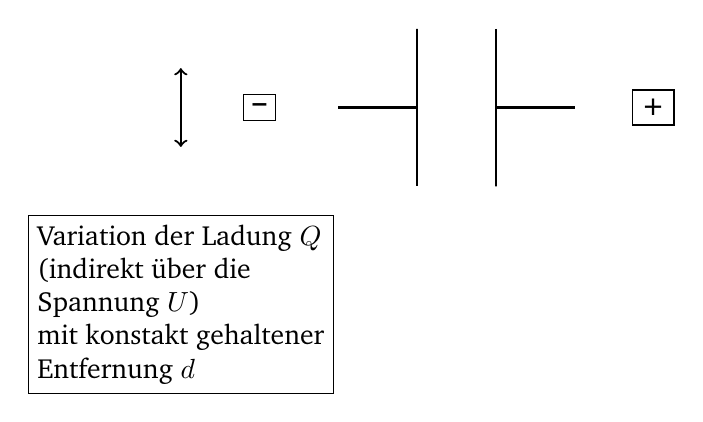
\begin{tikzpicture}
	    \draw[black,thick] (2,0) -- (3,0) -- (3,1) -- (3,-1);
	    \node[draw,align=left] at (1,0) {\textbf{--}};
	    \draw[black,thick] (4,1) -- (4,-1) -- (4,0) -- (5,0);
	    \node[draw,align=left] at (6,0) {\textbf{+}};
	    \draw[black,thick,<->] (0,-0.5) -- (0,0.5);
	    \node[draw,align=left] at (0,-2.5) {Variation der Ladung $Q$ \\ (indirekt über die\\ Spannung $U$) \\ mit konstakt gehaltener \\ Entfernung $d$};
	\end{tikzpicture}
	\\\\
	\begin{tabularx}{\textwidth}{|X|X|X|X|X|X|}
        \hline
        \textbf{U/kV} & 2 & 3 & 4 & 5 & 6 \\
        \hline
        \textbf{E/$\frac{kV}{m}$} & 90 & 140 & 180 & 210 & 240 \\
        \hline
	\end{tabularx}
	\\[1cm]
	\begin{tikzpicture}
	    \begin{axis}[
	        axis lines = left,
	        ylabel = $E/\frac{kV}{m}$,
	        xlabel = $U/kV$
	    ]
	        \addplot[
	            color=blue,
	            mark=square,
	            smooth,
	            thick
	        ] coordinates {
	            (2,90)(3,140)(4,180)(5,210)(6,240)
	        };
	    \end{axis}
	\end{tikzpicture}
	\\[1cm]
	Daraus folgt, dass $E$ proportional zu $U$ ist:
	\begin{align*}
	    E &\sim U
	\end{align*}
	Aus den vorherigen Erkenntnissen lässt sich nun Folgendes festhalten:
	\begin{align*}
	    E &\sim U \\
	    \xrightarrow[Proportionalitätsfaktor: 1] E&=\frac{U}{d} \\
	    \Rightarrow F_E &= \frac{U}{d} \cdot Q
	\end{align*}
	\subsection{Analogie}
	\begin{tikzpicture}
	    \draw[thick,orange] (2,2) -- (2,0) -- (0,0) -- (4,0);
	    \draw[thick,orange] (2,-4) -- (2,-2) -- (0,-2) -- (4,-2);
	    \filldraw[orange] (3.8,-1) circle (3pt);
	    \filldraw[orange] (3.3,-1.25) circle (3pt);
	    \filldraw[orange] (2.8,-1.5) circle (3pt);
	    \draw[thick,orange,->] (2.8,-1.6) -- (2.8,-2);
	    \draw[thick,orange,->] (3.3,-1.3) -- (3.3,-2);
	    \draw[thick,orange,->] (3.8,-1.1) -- (3.8,-2);
	    \node[draw,align=left,orange] at (4.5,-1.4) {$F_E$};
	    \draw[thick,black] (7,-1) -- (8,-1);
	    \filldraw[black] (7.5,0) circle (3pt);
	    \draw[thick,black,->] (7.5,0) -- (7.5,-0.75);
	    \node[draw,align=left] at (7.5,0.5) {$m$};
	    \node[draw,align=left] at (8.5,-0.5) {$F_G$};
	    \node[draw,align=left] at (7.5,-1.5) {Erde};
	\end{tikzpicture}
	\\\\
	Damit ist, weil die Kraft $F_E$ stets konstant und unabhängig vom Ort ist, nachgewiesen, dass - in vollständiger Analogie zum waagerechten Wurf im Schwerefeld der Erde - die Bahn des Elektrons parabelförmig sein muss.
\end{document}